%\pagestyle{fancy}
\chapter{Methods}
\label{ch:Methods}

\todoin{\begin{itemize}
    \item Coordinate system problem
    \item Problem with car tilt
    \item Short description of different methods
\end{itemize}}
\begin{figure}[htpb]
    \centering
	\documentclass[11pt]{standalone}
\usepackage{tikz}
\usetikzlibrary{angles, calc, decorations.pathmorphing, quotes, spy}

\begin{document}
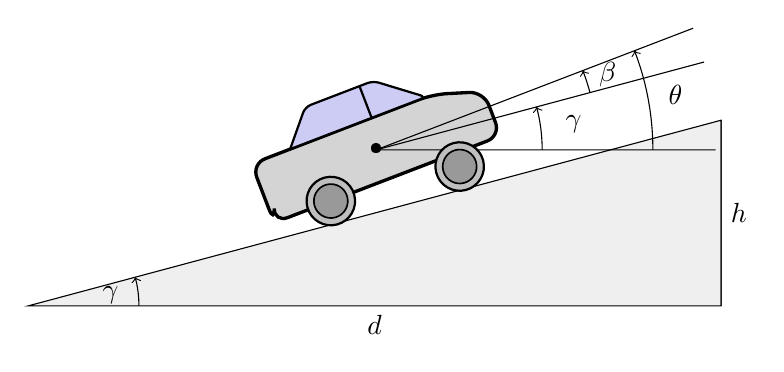
\begin{tikzpicture}[scale=.88]
    % Define/Calc ramp parameters
    % Ramp length
    \def\rl{10};
    % Ramp angle [deg]
    \def\ra{15};
    % Ramp height
    \def\rh{{tan(\ra)*\rl}};

    % RAMP
    % Define the points
    \coordinate (A) at (0,0);
    \coordinate (B) at ($(A) + (\rl,0)$);
    \coordinate (C) at ($(B) + (0,\rh)$);
    % Draw and fill ramp
    \filldraw[draw=black, fill=lightgray!25] (A) -- (B) -- (C) -- cycle;
    % Label length and draw angle
    \path (A) -- (B) node [midway, below] {$d$}
    pic[draw, ->, angle radius=40pt,
            angle eccentricity=0.75, "$\gamma$"]{angle=B--A--C};
    % Label height
    \draw (B) -- (C) node [midway, right] {$h$};

    % CAR
    % Tilt whole car
    \begin{scope}[scale=0.7, xshift=\rl*0.5 cm, yshift=1.9 cm, rotate=\ra]

        % Car height
        \def\ch{2}
        % Car length
        \def\cl{5}
        % Car body height
        \def\bh{\ch*0.65}
        % Roof length
        \def\rl{\cl*0.6}
        % Roof height
        \def\rh{\ch*0.35}
        % Car tilt angle
        \def\ct{6}

        % Tilt body without wheels
        \begin{scope}[rotate=\ct, yshift=-0.2cm]
            % Anchor point is southwest
            \coordinate (b) at (0,0);
            % Offset to roof and wheels
            \coordinate (r) at ($(b) +(\cl*0.17,\ch*0.65)$);
            \coordinate (w) at ($(b) + (\cl*0.25,0)$);
            % Body
            \draw[black, fill=black!17, rounded corners=1.2ex, very thick]
            (b) -- ++(0,\bh) -- ++(\cl*1/5,0) --  ++(\cl*3/5,0) -- ++(\cl*1/5,-\bh*0.25)
            -- ++(0, -\bh*0.75) -- (b) -- cycle;
            % Roof
            \draw[very thick, rounded corners=0.5ex, fill=black!20!blue!20!white,thick]
            (r) -- ++(0.2*\rl,\rh) -- ++(0.5*\rl,0) -- ++(0.3*\rl,-\rh) -- (r);
            \draw[thick] (r)++(\rl*0.6,0) -- ++(0,\rh);

            % Car middle point
            \coordinate (m) at (\cl*0.5, \bh*0.5);
            \node at (m) {\textbullet};
            % Line parallel to body
            \draw (m) -- ++(7,0) coordinate (pb);
            % Line parallel to ramp
            \draw[rotate = -\ct] (m) -- ++(7,0) coordinate (pr);
            % Line parallel to ground
            \draw[rotate = -\ct-\ra] (m) -- ++(7,0) coordinate (pg);
            % Draw angles
            \path (pb) -- (pr)
            pic[draw, ->, angle radius=60pt, angle eccentricity=1.2, "$\gamma$"] {angle = pg--m--pr}
            pic[draw, ->, angle radius=80pt, angle eccentricity=1.1, "$\beta$"] {angle = pr--m--pb}
            pic[draw, ->, angle radius=100pt, angle eccentricity=1.1, "$\theta$"] {angle = pg--m--pb};
        \end{scope}

        % Wheels
        \draw[draw=black,fill=gray!50,thick] (w) circle (.5);
        \draw[draw=black,fill=gray!50,thick] (w) ++(\cl*0.55,0) circle (.5);
        % Inner wheels
        \draw[draw=black,fill=gray!80,semithick] (w) circle (.35);
        \draw[draw=black,fill=gray!80,semithick] (w) ++(\cl*0.55,0) circle (.35);
    \end{scope}
\end{tikzpicture}
\end{document}
	\caption{Car driving on a ramp. Due to forward acceleration the car tilts back.}
	\label{fig:tikz_car_tilt}
\end{figure}


\section{IMU only}
\subsection{Calibration}
Because the measurements of the IMU are measured in the device frame $\mathcal{I}$, which is not aligned with the car frame $\mathcal{C}$, they have to be transformed.
This can be achieved using a rotation matrix \mtf{i}{c} $\in \mathbb{R}^{3\times3}$ which transforms the measurements of the linear acceleration $\vincs{a}{I}_n \in \mathbb{R}^{1\times3}$ and angular velocity ${\vincs{v}{I}_n \in \mathbb{R}^{1\times3}}$ into the car frame.
Note that the upper index? to the left of the matrix symbol denotes the source frame, whereas the destination frame is written below it.
 $n \in \mathbb{N}$ is the time step.\\
During standstill, the only measurable acceleration besides noise and bias is the acceleration due to gravity.
Assuming the car stands on flat ground, the gravity acceleration in the car frame is measured in upwards z-direction.
In a first step, the measured linear acceleration (gravity) in the IMU frame will be aligned with the z-axis of the car.
According to Euler's rotation theorem, which says that any arbitrary rotation of a rigid body while holding one point (origin) fixed can be achieved by a rotation around a single fixed axis passing through the origin, there exists one rotation axis $\mathbf{j}$ and rotation angle $\alpha$ to achieve this.\\
In the first step, the quaternion \qtf{i}{b} which describes the rotation from the device frame $\mathcal{I}$ to an intermediate coordinate system $\mathcal{B}$, which has the z-axis up, will be found.
Resulting in $\vincs{z}{b} = \vincs{z}{c} = \mathbf{e}_\mathrm{z} = \left(\begin{array}{lll} 0 & 0 & 1 \end{array}\right)^{\top}$.
Note that this is not necessarily true for the other axes, $\vincs{x}{b}\neq\vincs{x}{c}$ and $\vincs{z}{b}\neq\vincs{z}{c}$.\\
Using linear algebra \todo{better explaination} the rotation axis $\vb{j} \in \mathbb{R}^{1\times3}$, which is perpendicular to both \vincs{a}{i} and \vincs{z}{c}, can be found with
\begin{equation}
    \vb{j} = \frac{\vincs{\vu{a}}{i} \vdot \vincs{a}{c}}{\norm{\vincs{\vu{a}}{i} \cp \vincs{a}{c}}}
    = \frac{\vincs{\vu{a}}{i} \vdot \vb{e}_\mathrm{z} }{\norm{\vincs{\vu{a}}{i} \cp \vb{e}_\mathrm{z}}}
    = \frac{\vincs{\vu{a}_\mathrm{z}}{i}}{\norm{\vincs{\vu{a}_\mathrm{y}}{i}\vb{e}_\mathrm{x} - \vincs{\vu{a}_\mathrm{x}}{i}\vb{e}_\mathrm{y}}}
\end{equation}
with $\mathbf{a} \in \mathbb{R}^{1\times3}$ being the measured linear acceleration (average) in the IMU or car frame respectively and $\vu{a}$ being the unit vector of it.\\
The rotation angle can be calculated using
\begin{equation}
    \tan(\alpha) = \frac{\norm{\vincs{\vu{a}}{i} \cp \vb{e}_\mathrm{z}}}{\vincs{\vu{a}}{i} \vdot \vb{e}_\mathrm{z}} \implies
    \alpha = \arctan(\frac{\norm{\vincs{\vu{a}}{i} \cp \vb{e}_\mathrm{z}}}{\vincs{\vu{a}}{i} \vdot \vb{e}_\mathrm{z}})
\end{equation}
which results in combination with the rotation axis to the quaternion
\begin{equation}
    \qtf{i}{b} =
    \begin{bmatrix}
        \vb{j}\vdot\sin(\frac{\alpha}{2}) \\
        \cos(\frac{\alpha}{2})
    \end{bmatrix}
\end{equation}
\itodo{Decide for a notation (w,x,y,z is more common I think)}
Now that the z-axes of both frames are aligned, the x- and y-axis can be aligned by a rotation around the z-axis.
To find this rotation angle $\beta$, the car has to be accelerated forward.
This acceleration is being measured along the x- and y-axis.
The z-axis is set to zero, because it only measures the gravity which is not of interest.
The resulting vector is being aligned with the forward axis of the car $\vincs{x}{c} = \mathbf{e}_\mathrm{x} = \left(\begin{array}{lll} 1 & 0 & 0 \end{array}\right)^{\top}$, in the same way as before.
Resulting in the rotation angle
\begin{equation}
    \beta = \arctan(\frac{\norm{\vincs{\vu{a}}{b} \cp \vb{e}_\mathrm{x}}}{\vincs{\vu{a}}{b} \vdot \vb{e}_\mathrm{x}})
\end{equation}
The resulting quaternion
\begin{equation}
    \qtf{b}{c} =
    \begin{bmatrix}
        \vb{e}_\mathrm{z}\vdot\sin(\frac{\beta}{2}) \\
        \cos(\frac{\beta}{2})
    \end{bmatrix}
\end{equation}
can then be concatenated with the previous quaternion to get the final quaternion
\begin{equation}
    \qtf{i}{c} = \qtf{b}{c} \otimes  \qtf{i}{b}
\end{equation}
A quaternion of the form
$\mathbf{q} = \left[\begin{array}{llll} w & x & y & z \end{array}\right]^{\top}$
can be converted to a rotation matrix with
\begin{equation}
    % { }_{\mathcal{C}}^{\mathcal{I}} \mathbf{M} =
    \mathbf{M} =
    \left[
        \begin{array}{ccc}
            1-2 y^{2}-2 z^{2} & 2(x y-z w) & 2(x z+y w) \\
            2(x y+z w) & 1-2 x^{2}-2 z^{2} & 2(y z-x w) \\
            2(x z-y w) & 2(y z+x w) & 1-2 x^{2}-2 y^{2}
        \end{array}
        \right]
    \end{equation}
And finally the measurements $\mathbf{A}$ can be transformed using
\begin{equation}
    \vincs{A}{c} = \mtf{i}{c} \vdot \vincs{A}{i}
\end{equation}

\begin{figure}[htpb]
    \centering
    \documentclass{standalone}
\usepackage{tikz}
\usetikzlibrary{angles, calc, decorations.pathmorphing, quotes, spy}

\begin{document}
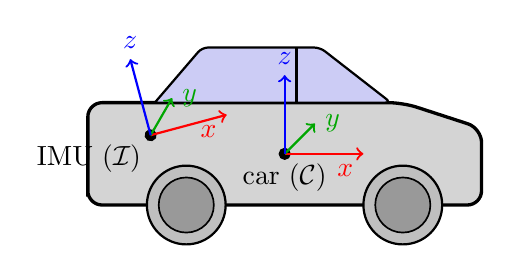
\begin{tikzpicture}[scale=1]
    % Define car parameters
    % Car height
    \def\ch{2}
    % Car length
    \def\cl{5}
    % Car body height
    \def\bh{\ch*0.65}
    % Roof length
    \def\rl{\cl*0.6}
    % Roof height
    \def\rh{\ch*0.35}
    % Car tilt angle
    \def\ct{6}
    % Anchor point is southwest
    \coordinate (b) at (0,0);
    % Offset to roof and wheels
    \coordinate (r) at ($(b) +(\cl*0.17,\ch*0.65)$);
    \coordinate (w) at ($(b) + (\cl*0.25,0)$);

    % Body
    \draw[black, fill=black!17, rounded corners=1.2ex, very thick]
    (b) -- ++(0,\bh) -- ++(\cl*1/5,0) --  ++(\cl*3/5,0) -- ++(\cl*1/5,-\bh*0.25)
    -- ++(0, -\bh*0.75) -- (b) -- cycle;
    % Roof
    \draw[very thick, rounded corners=0.5ex, fill=black!20!blue!20!white,thick]
    (r) -- ++(0.2*\rl,\rh) -- ++(0.5*\rl,0) -- ++(0.3*\rl,-\rh) -- (r);
    % \draw[thick] ($(r) + (\cl*0.5,\bh)$) -- ++(0,\rh);
    \draw[thick] (r)++(\rl*0.6,0) -- ++(0,\rh);

    % Wheels
    \draw[draw=black,fill=gray!50,thick] (w) circle (.5);
    \draw[draw=black,fill=gray!50,thick] (w) ++(\cl*0.55,0) circle (.5);
    % Inner wheels
    \draw[draw=black,fill=gray!80,semithick] (w) circle (.35);
    \draw[draw=black,fill=gray!80,semithick] (w) ++(\cl*0.55,0) circle (.35);

    % Car middle point
    \coordinate (m) at (\cl*0.5, \bh*0.5);
    \filldraw (m) circle (2pt) node[below] {car ($\mathcal{C}$)};
    % Coordinate frames
    \draw[thick,->, red] (m) -- ++(1,0,0) node[anchor=north east]{$x$};
    \draw[thick,->, black!35!green] (m) -- ++(0,0,-1) node[anchor=west]{$y$};
    \draw[thick,->, blue] (m) -- ++(0,1,0) node[anchor=south]{$z$};

    % IMU middle point (random)
    \begin{scope}[rotate=15]
        \coordinate (mi) at (\cl*0.2, \bh*0.5);
        \filldraw (mi) circle (2pt) node[below left] {IMU ($\mathcal{I}$)};
        % Coordinate frames
        \draw[thick,->, red] (mi) -- ++(1,0,0) node[anchor=north east]{$x$};
        \draw[thick,->, black!35!green] (mi) -- ++(0,0,-1) node[anchor=west]{$y$};
        \draw[thick,->, blue] (mi) -- ++(0,1,0) node[anchor=south]{$z$};
    \end{scope}
\end{tikzpicture}
\end{document}
	\caption{Coordinate frames (graphic might not be necessary)}
    \label{fig:tikz_car_frames}
\end{figure}

\subsection{Linear acceleration only}


\subsection{Angular velocity only}


\subsection{Complementary filter}
\itodo{Or is combination of linear acceleration and angular velocity not already sensor fusion?}



\section{LiDAR only}
\subsection{Calibration}
\itodo{Describe lidar calibration algorithm}
A flow chart of the described algorithm is shown in figure \ref{fig:lidarCalibration}.
\itodo{Not sure if flow chart is best way to help understand explaination. Algorithm pseudo code might be better}
\begin{figure}[htb]
	\centering
	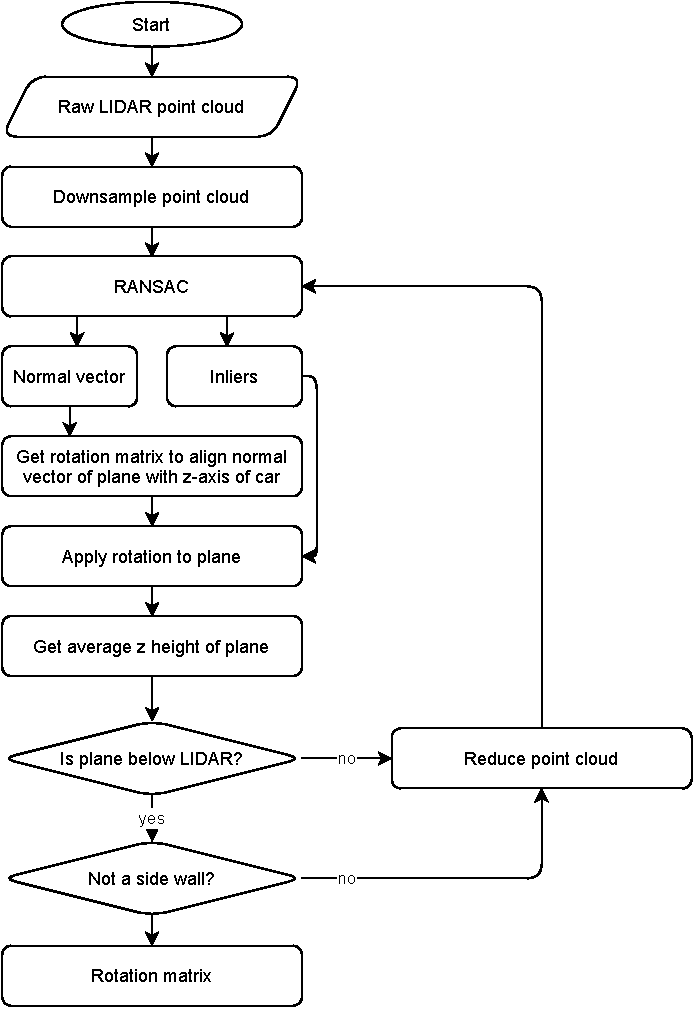
\includegraphics[width=0.7\linewidth]{lidarCalibration.pdf}
	\caption{Algo for lidar alignment}
	\label{fig:lidarCalibration}
\end{figure}


\subsection{Algo description (Only have one)}
\itodo{Probably add flow chart / pseudo-code algorithm as well}



\section{Camera only}



\section{Sensor fusion}
\itodo{Brief explaination what sensor fusion is and why useful}


\subsection{IMU and Odometer}

\subsubsection{Car acceleration from odometer data}
Because the odometer only delivers the speed of each wheel, the car velocity has to be calculated first.
During turns the left and right wheels travel at different speeds, the wheel on the inner side of the turn travels slower, than the outer wheel.
E.g. during a left turn, the left wheel moves slower than the right wheel.
A simple yet sufficiently accurate model to calculate the car velocity from the wheel speeds is the linear single track model ("Einspurmodell") \cite{Mitschke2014}.
In this model both wheels on one axis are replaced with one wheel in the middle.
\itodo{Explain model}
The linear assumption holds true for low lateral accelerations (up to \SI{4}{\metre\per\second}), which will not be surpassed in the parking garage scenario.
Using the assumptions from above, the car velocity $v_\mathrm{car}(t)$ can be calculated with
\begin{align}
    \alpha(t) &= \frac{v_\mathrm{rl}(t) - v_\mathrm{rr}(t)}{d} \\
    \gamma(t) &= \frac{\alpha(t)}{f_\mathrm{odom}} \\
    v_\mathrm{car}(t) &= \frac{v_\mathrm{rl}(t) + v_\mathrm{rr}(t)}{2}\cdot\cos(\gamma)
\end{align}
with $v_\mathrm{rl} \text{ and } v_\mathrm{rr}$ being the wheel speeds of the rear right and rear left wheel respectively.
$\alpha$ is a helper variable \todo{I can't explain it well}, $d$ the track width! and $\gamma$ is the yaw angle of the car.\\
The car's acceleration can be derived from the velocity using
\begin{equation}
    a_\mathrm{car}(t) = \dv{t}v_\mathrm{car}.
\end{equation}
But because all measurements are discrete, numerical differentiation e.g. forward difference must be used
\begin{equation}
    a_\mathrm{car}(h) = \frac{v_\mathrm{car}(x + h) - v_\mathrm{car}(x)}{h}
\end{equation}
with $h$ being the step size, which depends on the rate of the sensor.

\subsubsection{Gravity method}
\begin{figure}[htpb]
    \centering
    \documentclass[12pt]{standalone}
\usepackage{tikz}
\usetikzlibrary{angles, calc, decorations.pathmorphing, quotes, spy}

\begin{document}
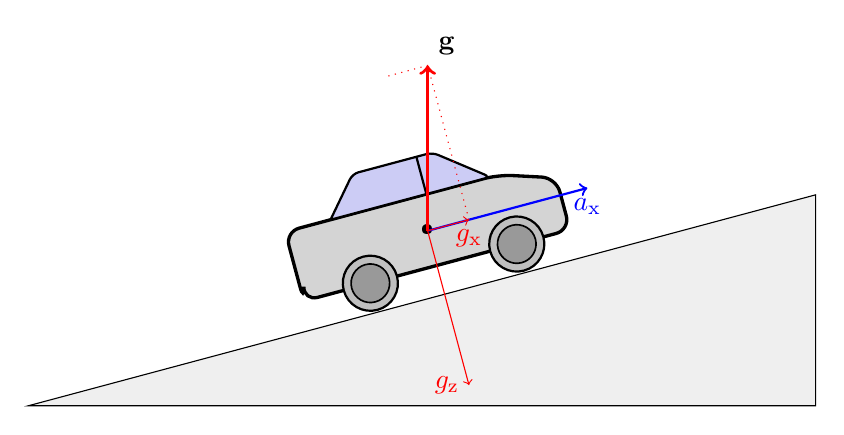
\begin{tikzpicture}[scale=1]
    % Define/Calc ramp parameters
    % Ramp length
    \def\rl{10};
    % Ramp angle [deg]
    \def\ra{15};
    % Ramp height
    \def\rh{{tan(\ra)*\rl}};

    % RAMP
    % Define the points
    \coordinate (A) at (0,0);
    \coordinate (B) at ($(A) + (\rl,0)$);
    \coordinate (C) at ($(B) + (0,\rh)$);
    % Draw and fill ramp
    \filldraw[draw=black, fill=lightgray!25] (A) -- (B) -- (C) -- cycle;

    % CAR
    % Tilt whole car
    \begin{scope}[scale=0.7, xshift=\rl*0.5 cm, yshift=1.9 cm, rotate=\ra]
        % Car height
        \def\ch{2}
        % Car length
        \def\cl{5}
        % Car body height
        \def\bh{\ch*0.65}
        % Roof length
        \def\rl{\cl*0.6}
        % Roof height
        \def\rh{\ch*0.35}
        % Car tilt angle
        \def\ct{6}

        % Anchor point is southwest
        \coordinate (b) at (0,0);
        % Offset to roof and wheels
        \coordinate (r) at ($(b) +(\cl*0.17,\ch*0.65)$);
        \coordinate (w) at ($(b) + (\cl*0.25,0)$);
        % Body
        \draw[black, fill=black!17, rounded corners=1.2ex, very thick]
        (b) -- ++(0,\bh) -- ++(\cl*1/5,0) --  ++(\cl*3/5,0) -- ++(\cl*1/5,-\bh*0.25)
        -- ++(0, -\bh*0.75) -- (b) -- cycle;
        % Roof
        \draw[very thick, rounded corners=0.5ex, fill=black!20!blue!20!white,thick]
        (r) -- ++(0.2*\rl,\rh) -- ++(0.5*\rl,0) -- ++(0.3*\rl,-\rh) -- (r);
        \draw[thick] (r)++(\rl*0.6,0) -- ++(0,\rh);

        % % Car middle point
        \coordinate (m) at (\cl*0.5, \bh*0.5);
        \node at (m) {\textbullet};
        % Wheels
        \draw[draw=black,fill=gray!50,thick] (w) circle (.5);
        \draw[draw=black,fill=gray!50,thick] (w) ++(\cl*0.55,0) circle (.5);
        % Inner wheels
        \draw[draw=black,fill=gray!80,semithick] (w) circle (.35);
        \draw[draw=black,fill=gray!80,semithick] (w) ++(\cl*0.55,0) circle (.35);

        % Draw car acceleration
        \draw[blue, thick, ->] (m) -- ++(3,0) node[anchor=north]{$a_\mathrm{x}$};
        % Gravity vectors
        % Length of g vector
        \def\gl{3}
        % Length of g vector components
        \def\gxl{{\gl*sin(\ra)}}
        \def\gzl{{\gl*cos(\ra)}}
        % Draw vectors
        \draw[red, ->, very thick, rotate=-\ra] (m) -- ++(0,\gl) node[anchor=south west, black](g_end){$\mathbf{g}$};
        \draw[red, thin, ->] (m) -- ++(\gxl,0) node[anchor=north]{$g_\mathrm{x}$};
        \draw[red, thin, ->] (m) -- ++(0,-\gzl) node[anchor=east]{$g_\mathrm{z}$};
        \draw[red, dotted] ($(m)+(\gxl,0)$) -- ++(0,\gzl) -- ++(-\gxl,0);
    \end{scope}
\end{tikzpicture}
\end{document}
    \caption{Gravity measured by IMU (in car frame). Show that $g_z$ etc}
    \label{fig:tikz_car_gravity}
\end{figure}
\todoin{\begin{itemize}
    \item Algo description
    \item Problems
\end{itemize}
}


\subsection{IMU and odometer and LiDAR}
\todoin{\begin{itemize}
    \item Algo description
\end{itemize}
}